\documentclass[crop,tikz]{standalone}
\usepackage{tikz}
	\usetikzlibrary{shapes}
	\usetikzlibrary{automata}
	\usetikzlibrary{arrows}
	\usetikzlibrary{backgrounds}
	\usetikzlibrary{calc}
	\usetikzlibrary{positioning}
	\usetikzlibrary{patterns}
	\usetikzlibrary{decorations.pathmorphing}
	\usetikzlibrary{decorations.pathreplacing}


\usepackage[scaled]{helvet}
\renewcommand{\familydefault}{\sfdefault}
	
\input{../../../../../resources/latex/_symbols.qmd}
\begin{document}

\begin{tikzpicture}

    \pgfdeclarelayer{background layer}
    \pgfdeclarelayer{foreground layer}
    \pgfsetlayers{background layer,main,foreground layer}

    \node (2d) at (0pt,0pt) {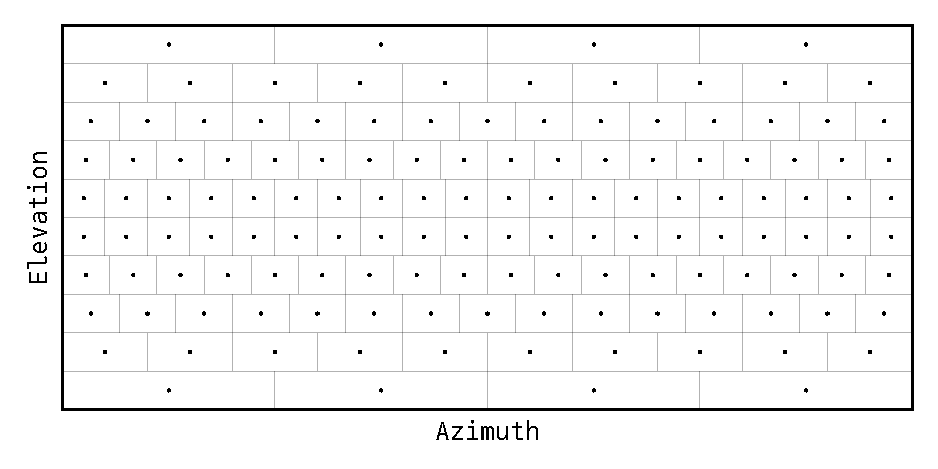
\includegraphics[width=0.5\textwidth]{./gs2dgrid_reduced_2d.pdf}};
    \node[below right = 0 and -3.7 of 2d] (proj) {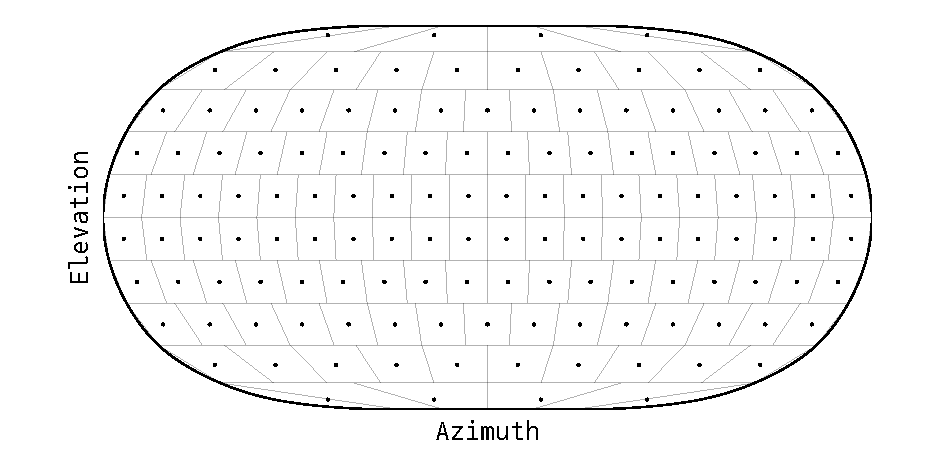
\includegraphics[width=0.5\textwidth]{./gs2dgrid_reduced_proj.pdf}};
    
    \begin{pgfonlayer}{background layer}
        \node[below right = -1.4 and -1.5 of proj] (3d) {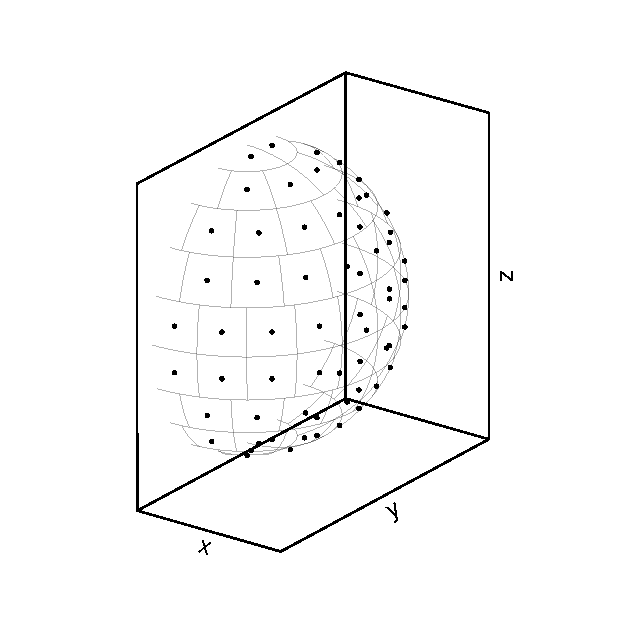
\includegraphics[width=0.4\textwidth, trim={0 30pt 0 0}, clip]{./gs2dgrid_reduced_3d.pdf}};
    \end{pgfonlayer}

    \draw[-latex, very thick] (3d.70) to [in=0, out=90] node[near end, xshift=0, yshift=20]{\footnotesize{spherical projection}} (2d.15);
    
    \draw[-latex, very thick] (2d.220) to [in=180, out=270] node[near end, xshift=20, yshift=-25]{\footnotesize{cartesian projection}} (3d.190);

\end{tikzpicture}

\end{document}